\documentclass{beamer}
\usetheme{Dresden} % My favorite!
\usecolortheme{beaver} % Simple and clean template
\usepackage{amssymb,latexsym}
\usepackage{xltxtra, xgreek}
\usepackage[boxed]{algorithm2e}
\usepackage{float}
\usepackage{textcomp}
\usepackage{url} 
\usepackage{ocamldoc}			
\setsansfont[Mapping=tex-text]{CMU Concrete}
\setmonofont{Courier New}
\SetKw{Kwdto}{downto}

%\usetheme{Boadilla} % Pretty neat, soft color.
%\usetheme{default}
%\usetheme{Warsaw}
%\usetheme{Bergen} % This template has nagivation on the left
%\usetheme{Frankfurt} % Similar to the default 
%with an extra region at the top.
%\usecolortheme{seahorse} % Simple and clean template
%\usetheme{Darmstadt} % not so good
% Uncomment the following line if you want %
% page numbers and using Warsaw theme%
% \setbeamertemplate{footline}[page number]
\setbeamercovered{transparent}
%\setbeamercovered{invisible}
% To remove the navigation symbols from 
% the bottom of slides%
\setbeamertemplate{navigation symbols}{} 
\expandafter\def\expandafter\insertshorttitle\expandafter{%
  \insertshorttitle\hfill\insertframenumber\,/\,\inserttotalframenumber}
  

   
  

%\usepackage{bm}         % For typesetting bold math (not \mathbold)
%\logo{\includegraphics[height=0.6cm]{yourlogo.eps}}
%
\title[Elliptic Curve Cryptography]{Υλοποίηση ανταλλαγής κλειδιού DH και ψηφιακών υπογραφών βασισμένη σε ελλειπτικές καμπύλες}
\author{Νίκος Γιανναράκης \\ \and Ζωή Παρασκευοπούλου}

\institute[]
{
Σχολή Ηλεκτρολόγων Μηχανικών και Μηχανικών Υπολογιστών\\
Εθνικό Μετσόβιο Πολυτεχνείο
}
\date{\today}
\begin{document}

\begin{frame}
\titlepage
\end{frame}
\begin{frame}
\frametitle{Κρυπτογραφία με ελλειπτικές καμπύλες}
\begin{block}
{Why elliptic curve cryptography?}
\begin{itemize}
\item Αυξημένη ασφάλεια με μικρότερα μεγέθη κλειδιών
\item Μειωμένο υπολογιστικό κόστος και bandwitdh
\item Ιδανικές για φορητές συσκευές λόγω ενεργειακών απαιτήσεων (κινητά κλπ.)
\item ECC σε secure web servers, επιτάχυνση εως και $280\%$ \cite{SUN}
\end{itemize}
\end{block}
\end{frame}

%
\begin{frame}
\frametitle{Σύγκριση μήκους κλειδιού}
\begin{figure}
\begin{center}
\begin{tabular}{|l|l|l|l|} \hline
\textbf{ECC} & \textbf{RSA} & \textbf{Αναλογία} & \textbf{AES} \\ \hline
160 & 1024 & 1:6 & \\ \hline
256 & 3072 & 1:12 & 128 \\ \hline
384 & 7680 & 1:20 & 192 \\ \hline
512 & 15360 & 1:30 & 256 \\ \hline
\end{tabular}
\end{center}
\caption{Σύγκριση μήκους κλειδιού σε bits}
\end{figure}

\begin{figure}
\begin{center}
\begin{small}
\begin{tabular}{|l|l|l|} \hline
& \textbf{ECC-160 \hspace{1em} RSA-1024} & \textbf{ECC-224 \hspace{1em} RSA-2048}\\ \hline
Time(ms) & \hspace{1em} 3.69 \hspace{4.5em} 8.75 & \hspace{1em} 5.12 \hspace{4.5em} 56.18 \\ \hline
Ops/Sec  & \hspace{1em} 271.3 \hspace{4em} 114.3 & \hspace{1em} 195.5 \hspace{4.3em} 17.8 \\ \hline
Perf ratio  & \hspace{3.5em} 2.4 : 1.0 & \hspace{3.5em} 11.0 : 1.0 \\ \hline
Key ratio  & \hspace{3.5em} 1.0 : 6.4 & \hspace{3.5em} 1.0 : 9.1 \\ \hline
\end{tabular}
\end{small}
\end{center}
\caption{Σύγκριση απόδοσης ανάλογα με το μήκος κλειδιού \cite{SUN}}
\end{figure}

\end{frame}

\begin{frame}
\frametitle{Ελλειπτικές καμπύλες στο $\mathcal{R}$}
\begin{block}
{Ορισμός}
Μία ελλειπτική καμπύλη στο $\mathcal{R}$ μπορεί να οριστεί ως το σύνολο των σημείων (x,y) που ικανοποιούν μία εξίσωση ελλειπτικής καμπύλης της μορφής: 
$$y^2 = x^3 + a \cdot x + b \; , \; x,y,a,b \in \mathcal{R}$$
μαζί με ένα σημείο $\mathcal{O}$, το οποίο ονομάζουμε σημείο στο άπειρο.
\end{block}
\begin{block}
{Ορισμός πράξεων}
\begin{itemize}
\item Πρόσθεση δύο σημείων $P,Q$
\item Διπλασιασμός ενός σημείου $P$
\end{itemize}
\end{block}
\end{frame}


%
\begin{frame}
\frametitle{Πρόσθεση δύο σημείων πάνω σε ελλειπτικές καμπύλες στο $\mathcal{R}$}
H πρόσθεση δύο σημείων $P, Q$ μπορεί να οριστεί γεωμετρικά
\begin{center}
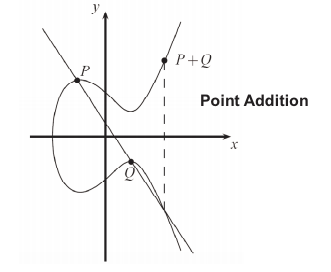
\includegraphics[scale=0.5]{add.png}

\end{center}\end{frame}

%
\begin{frame}
\frametitle{Διπλασιασμός σημείου πάνω σε ελλειπτικές καμπύλες στο $\mathcal{R}$}
Ο διπλασιασμός ενός σημείου πάνω σε μία ελλειπτική καμπύλη ορίζεται γεωμετρικά σύμφωνα με το παρακάτω σχήμα
\begin{center}
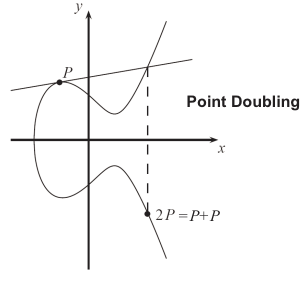
\includegraphics[scale=0.5]{double.png}

\end{center}\end{frame}

%
\begin{frame}
\begin{block}
{Προβλήματα}
\begin{itemize}
\item Αργές πράξεις σε πραγματικούς αριθμούς
\item Έλλειψη ακρίβειας
\end{itemize}
\end{block}
\end{frame}

%
\begin{frame}
\frametitle{Ελλειπτικές καμπύλες πάνω από το $\mathbb{F}_p$ και το $\mathbb{F}_{2^m}$}
\begin{block}
{Ορισμός}
Διαλέγοντας $a,b \in \mathbb{F}_p$  και υπολογίζοντας τα σημεία $(x,y)$ της καμπύλης $modulo \; p$ ορίζουμε μία ελλειπτική καμπύλη στο $\mathbb{F}_p$.
\end{block}
\end{frame}

%
\begin{frame}
\frametitle{Πρόσθεση δύο σημείων πάνω σε ελλειπτικές καμπύλες στο $\mathbb{F}_p$}
H πρόσθεση δύο σημείων $R = P + Q$ σε μία ελλειπτική καμπύλη στο $\mathbb{F}_p$ ορίζεται αλγεβρικά:
 \begin{align*}
 & s = \frac{(y_P - y_Q)}{(x_P - x_Q)}  \pmod p \\
 & x_R = s^2 - x_P - x_Q \pmod p \\
 & y_R = -y_P + s \cdot (x_P - x_R) \pmod p
 \end{align*}
 \medskip
 Το $\mathcal{O}$ είναι το ουδέτερο στοιχείο της πρόσθεσης : $P + \mathcal{O} = P$.
\end{frame}

%
\begin{frame}
\frametitle{Διπλασιασμός σημείου πάνω σε ελλειπτικές καμπύλες στο $\mathbb{F}_p$}
Ο διπλασιασμός σημείου $R = 2P$ σε μία ελλειπτική καμπύλη στο $\mathbb{F}_p$ ορίζεται αλγεβρικά:
 \begin{align*}
  & s = \frac{(3 \cdot x^2_P + a)}{2 \cdot y_P} \pmod p \\
  & x_R = s^2 - 2 \cdot x _P \pmod p \\
  & y_R = -y_p + s \cdot (x_P - x_R) \pmod p
 \end{align*}
\end{frame}

%
\begin{frame}
\frametitle{Βαθμωτός πολλαπλασιασμός πάνω σε ελλειπτικές καμπύλες στο $\mathbb{F}_p$}
Με χρήση των παραπάνω πράξεων μπορούμε να ορίσουμε την πράξη του βαθμωτού πολλαπλασιασμού $R = k \cdot P$ όπου $l \in \mathbb{Z}$ και $P$ ένα σημείο ελλειπτικής καμπύλης.
$P = \mathcal{O} \rightarrow k \cdot P = \mathcal{O}$
\begin{itemize}
\item Naive $P + P  \ldots + P$
\item Double-and-add (το ανάλογο του επαναλαμβανόμενου τετραγωνισμού)
\item Windowed, Sliding-window, wNAF, \\ Montogomery ladder $\ldots$ \cite{BERN}
\end{itemize}
\end{frame}

%
\begin{frame}
\frametitle{Double-and-add}
\begin{algorithm}[H]
\SetAlgoNoLine 
 \KwIn{Elliptic curve $E$, elliptic curve point $P$, scalar $d$:  $(d_1 d_2 \ldots d_t)$ }
 \KwOut{$T = d \cdot P$ }
 $T \leftarrow P$ \\
 \For{$i \leftarrow t -1$ \Kwdto $0$}{
 	$T \leftarrow T + T \pmod n$\\
 	\If{$d_i = 1$}{$T \leftarrow T + P \pmod n$}
 } 
 \KwRet{T}
\caption{Μέθοδος double-and-add}
\end{algorithm}
\end{frame}

%
\begin{frame}
\frametitle{Το πρόβλημα του διακριτού λογαρίθμου σε ελλειπτικές καμπύλες (ECDLP)}
\begin{block}
{Ορισμός}
'Εστω ελλειπτική καμπύλη  στο $\mathbb{F}_p$ και έστω δύο σημεία αυτής $P,Q$. Αν η τάξη του $P$ είναι $n$ τότε το πρόβλημα διακριτού λογαρίθμου ορίζεται ως η εύρεση ενός ακεραίου $ 0 \leq l \leq n -1$ τέτοιου ώστε $Q = l \cdot P$.
\end{block}
\end{frame}

%
\begin{frame}
\frametitle{Ανταλλαγή κλειδιού με τη μέθοδο Diffie-Hellman για ελλειπτικές καμπύλες (ECDH)}
\begin{itemize}
\item Ο χρήστης Α και ο χρήστης Β επιλέγουν δημόσια τις παραμέτρους $D = (q, a, b, G, n, h)$
\item Ο χρήστης Α επιλέγει έναν τυχαίο αριθμό $1 \leq a \leq n -1$ υπολογίζει το $a \cdot G$ και το στέλνει στον B.
\item Ο χρήστης Β επιλέγει έναν τυχαίο αριθμό $1 \leq b \leq n -1$ υπολογίζει το $b \cdot G$ και το στέλνει στον Α.
\item Ο Α υπολογίζει το $a \cdot b \cdot G$
\item  Ο Β υπολογίζει το $b \cdot a \cdot G$
\item Το κοινό κλειδί τους είναι το $a \cdot b \cdot G = b \cdot a \cdot G$
\end{itemize}
\end{frame}

%
\begin{frame}
\frametitle{Ψηφιακές υπογραφές με τον αλγόριθμο DSA για ελλειπτικές καμπύλες (ECDSA)}
\begin{block}
{Παραγωγή υπογραφής}
Για να υπογράψει ένα μήνυμα $m$, ο χρήστης Α με παραμέτρους $D = (q, a, b, G, n, h)$ και ένα ζεύγος ιδιωτικού-δημόσιου κλειδιού $(d, Q)$ ακολουθεί τα παρακάτω βήματα
\end{block}
\end{frame}

%
\begin{frame}
\frametitle{Ψηφιακές υπογραφές με τον αλγόριθμο DSA για ελλειπτικές καμπύλες (ECDSA)}
\begin{block}
{Παραγωγή υπογραφής}
\begin{small}
\begin{enumerate}
\item Επιλέγει έναν τυχαίο αριθμό $k$ τέτοιο ώστε $1 \leq k \leq n-1$.
\item Υπολογίζει το σημείο $k \cdot G = (x_1, y_1)$.
\item Υπολογίζει το $r = x_1 \pmod n$. Αν $r = 0$ επιστρέφει στο βήμα $1$.
\item Υπολογίζει το $k^{-1} \pmod n$.
\item Υπολογίζει το $SHA-1(m)$ και μετατρέπει το αποτέλεσμα του bit-string σε έναν ακέραιο $e$.
\item Υπολογίζει το $s = k^{-1} \cdot (e + d \cdot r) \pmod n$. Αν $s = 0$ επιστρέφει στο βήμα $1$.
\item Η υπογραφή του A για το μήνυμα $m$ είναι $(r,s)$.
\end{enumerate}
\end{small}
\end{block}
\end{frame}

%
\begin{frame}
\frametitle{Ψηφιακές υπογραφές με τον αλγόριθμο DSA για ελλειπτικές καμπύλες (ECDSA)}
\begin{block}
{Επαλήθευση υπογραφής}
Για να επαληθεύσει μία υπογραφή $(r,s)$ σε ένα μήνυμα $m$, ο χρήστης Β παίρνει τις παραμέτρους $D = (q, FR, a, b, G, n, h)$ και το δημόσιο κλειδί $Q$ του Α και ακολουθεί τα παρακάτω βήματα:
\end{block}
\alert{Προσοχή! Ο Β θα πρέπει να ελέγξει ότι τα στοιχεία του Α δεν έχουν αλλοιωθεί, π.χ. αν το σημείο Q ανήκει στην καμπύλη που ορίζεται απο το D}
\end{frame}

%
\begin{frame}
\frametitle{Ψηφιακές υπογραφές με τον αλγόριθμο DSA για ελλειπτικές καμπύλες (ECDSA)}
\begin{block}
{Επαλήθευση υπογραφής}
\begin{small}
\begin{enumerate}
\item Επιβεβαιώνει ότι τα $r,s$ είναι ακέραιοι στο διάστημα $[1, n-1]$.
\item Υπολογίζει το $SHA-1(m)$ και μετατρέπει το αποτέλεσμα του bit-string σε έναν ακέραιο $e$.
\item Υπολογίζει το $w = s^{-1} \pmod n$.
\item Υπολογίζει το $u_1 = e \cdot w \pmod n$ και το $u_2 = r \cdot w \pmod n$.
\item Υπολογίζει το $X = u_1 \cdot G + u_2 \cdot G$
\item Εάν $X = \mathcal{O}$ τότε απορρίπτει την υπογραφή. Αλλιώς υπολογίζει τo $u = x_1 \pmod n$ όπου $x_1$ η συντεταγμένη $x$ του $X$. 
\item Δέχεται την υπογραφή αν και μόνο αν $u = r$.
\end{enumerate}
\end{small}
\end{block}
\end{frame}

%
\begin{frame}
\frametitle{Υλοποίηση}
\begin{block}
{Επιλογή παραμέτρων}
\begin{figure}[!htbp]
\begin{center}
\begin{tabular}{|l|l|} \hline
\textbf{Παράμετρος} & \textbf{Περιγραφή} \\ \hline
p & Η χαρακτηριστική του πεπερασμένου σώματος $\mathbb{F}_p$ \\ \hline
a & Ο συντελεστής a της ελλειπτικής καμπύλης \\ \hline
b & Ο συντελεστής b της ελλειπτικής καμπύλης \\ \hline
G & Ένα σημείο $G = (x_G, y_G)$  \\ \hline
n & Η τάξη του στοιχείου $G$ \\ \hline
h & $\sharp E(\mathbb{F}_p)/n$ \\ \hline
\end{tabular} \\
\end{center}
\caption{Domain Parameters}
\end{figure}
\alert{Απαιτείται πολύ προσεκτική επιλογή των παραμέτρων} \cite{ECDSA} \cite{SEC2} \cite{BPOOL}
\end{block}
\end{frame}

%
\begin{frame}
\frametitle{Υλοποίηση}
\begin{block}
{Επίπεδα υλοποίησης}
\begin{itemize}
\item Αριθμητική modulo με υποστήριξη για μεγάλους αριθμούς
\item Υλοποίηση των πράξεων που ορίζονται στην ομάδα (πρόσθεση, διπλασιασμός)
\item Υλοποίηση του βαθμωτού πολλαπλασιασμού
\item Υλοποίηση ενός κρυπτοσυστήματος π.χ. ECDH 
\end{itemize}
\end{block}
\end{frame}

%
\begin{frame}
\frametitle{Υλοποίηση στη γλώσσα OCaml}
\begin{block}
{Why OCaml?}
\begin{itemize}
\item \textbf{Μείωση σφαλμάτων.} Έλεγχος τύπων κατά τη μεταγλώττιση.
\item \textbf{Βιβλιοθήκες.} Αρκετές έτοιμες συναρτήσεις (για big numbers κ.α.)
\item \textbf{Ταχύτητα.} Απόδοση αρκετά κοντά σε low-level γλώσσες όπως C.
\item \textbf{Garbage collected.} Η διαχείριση μνήμης γίνεται αυτόματα, ένα πράγμα λιγότερο για να ανησυχούμε.
\end{itemize}
\end{block}
\begin{flushright}

\includegraphics[scale=0.7]{ocaml_logo.png}
\end{flushright}
\end{frame}

%
\begin{frame}
\frametitle{Υλοποίηση στη γλώσσα OCaml}
\begin{block}
{Βασικοί τύποι}
\label{type:Ecc.Ecc.point}\begin{ocamldoccode}
type point =
   Infinity
  | Point of Z.t * Z.t
\end{ocamldoccode}
\begin{ocamldocdescription}
An elliptic curve point. It is either infinity or a point (x,y).
\end{ocamldocdescription}
\index{point@\verb`point`}


\label{type:Ecc.Ecc.elliptic-underscorecurve}\begin{ocamldoccode}
type elliptic\_curve = {\char123}\\
  p : Z.t ;\\
  a : Z.t ;\\
  b : Z.t ;\\
  g : point ;\\
  n : Z.t ;\\
  h : Z.t ;\\
{\char125}
\end{ocamldoccode}
\index{elliptic-underscorecurve@\verb`elliptic_curve`}
\begin{ocamldocdescription}
The type of domain parameters
\end{ocamldocdescription}
\end{block}
\end{frame}

%
\begin{frame}
\frametitle{Υλοποίηση στη γλώσσα OCaml}
\begin{block}
{Modulo αριθμητική}
Χρησιμοποιήθηκε η βιβλιοθήκη μεγάλων αριθμών Zarith, χρησιμοποιεί το GMP (C/C++). Διάφορες ετοιμες συναρτήσεις για βασικές πράξεις όπως εύρεση αντιστρόφου ενός αριθμού $modulo \; n$. 
\end{block}
\end{frame}

%
\begin{frame}
\frametitle{Υλοποίηση στη γλώσσα OCaml}
\begin{block}
{Υλοποίηση πράξεων ομάδας}
\label{val:Ecc.Ecc.add-underscorepoint}\begin{ocamldoccode}
val add\_point : point -> point -> elliptic\_curve -> point
\end{ocamldoccode}
\index{add-underscorepoint@\verb`add_point`}
\begin{ocamldocdescription}
Given two points P and Q, both on the same elliptic curve, and the elliptic curve returns P+Q on that curve.
\end{ocamldocdescription}
\label{val:Ecc.Ecc.double-underscorepoint}\begin{ocamldoccode}
val double\_point : point -> elliptic\_curve -> point
\end{ocamldoccode}
\index{double-underscorepoint@\verb`double_point`}
\begin{ocamldocdescription}
Given a point P on an elliptic curve and the elliptic curve retuns the point 2P on that curve.
\end{ocamldocdescription}
\end{block}
\end{frame}

%
\begin{frame}
\frametitle{Υλοποίηση στη γλώσσα OCaml}
\begin{block}
{Υλοποίηση βαθμωτού πολλαπλασιασμού}
\label{val:Ecc.Ecc.multiply-underscorepoint}\begin{ocamldoccode}
val multiply\_point : point -> Z.t -> elliptic\_curve -> point
\end{ocamldoccode}
\index{multiply-underscorepoint@\verb`multiply_point`}
\begin{ocamldocdescription}
Given a point P on an elliptic curve, an integer k and the elliptic curve returns the scalar multiplication kP on that curve.
\end{ocamldocdescription}
\end{block}
\end{frame}

%
\begin{frame}
\frametitle{Βελτιστοποίησεις}
\begin{block}
{Βελτιστοποίηση αριθμητικής modulo}
Το πιο χρονοβόρο κομμάτι είναι οι πράξεις με μεγάλους αριθμούς και η αριθμητική modulo. Η χρήση της βιβλιοθήκης Zarith μας λύνει το πρόβλημα βελτιστοποίησεις αυτού του κομματιού καθώς χρησιμοποιεί το GMP που έχει γρήγορες υλοποιήσεις πράξεων στη γλώσσα C.
\end{block}
\begin{block}
{Βελτιστοποίηση πράξεων}
Οι συναρτήσεις add\_point και double\_point δεν παρουσιάζουν ιδιαίτερα περιθώρια βελτιστοποίησης. Μπορούμε να βελτιστοποιήσουμε τη συνάρτηση multiply\_point χρησιμοποιώντας έναν καλύτερο αλγόριθμο από αυτούς που έχουν αναφερθεί (η υλοποίηση μας χρησιμοποιεί τη μέθοδο double-and-add)
\end{block}
\end{frame}

%
\begin{frame}
\frametitle{Επιθέσεις}
\begin{itemize}
\item Επίλυση ECDLP (πρακτικά ανέφικτο με κατάλληλη επιλογή παραμέτρων)
\item Επίθεση στη συνάρτηση κατακερματισμού (hash function) εαν χρησιμοποιείται.
\item  Κακή διαχείριση κλειδιών (private key, αριθμός $k$ στο ECDSA) κλπ.
\end{itemize}
\end{frame}

%
\begin{frame}
\frametitle{Επίλυση του ECDLP}
\begin{block}
{Certicom ECC Challenge}
\begin{itemize}
\item Στόχος είναι να βρεθούν τα ιδιωτικά κλειδιά απο μία δοθείσα λίστα με δημόσια κλειδιά και τις αντίστοιχες παραμέτρους.
\item Επίπεδο 1 : 109-bit, 131-bit
\item Επίπεδο 2 : 163-bit, 191-bit, 239-bit, 359-bit
\item Το 2004 λύθηκε το πρόβλημα για τα 109-bit από $10000$ υπολογιστές σε 549 μέρες χρησιμοποιώντας τη μέθοδο rho. Για τα 131-bit όμως θα χρειαστούν σημαντικά περισσότεροι πόροι.
\item Τα προβλήματα στο επίπεδο 2 θεωρούνται υπολογιστικά ανέφτικα.
\end{itemize}
\end{block}
\end{frame}

%
\begin{frame}
\frametitle{Επίθεση στο ECDSA}
\begin{block}
{Sony Playstation 3}
Το playstation 3 χρησιμοποιεί το σχήμα ψηφιακής υπογραφής ECDSA για ψηφιακές υπογραφές στα παιχνίδια και στις αναβαθμίσεις του firmware του έτσι ώστε να μην επιτρέπεται σε unsigned κώδικα να εκτελεστεί στην κονσόλα.
\end{block}
\end{frame}

%
\begin{frame}
\frametitle{Επίθεση στο ECDSA}
\begin{block}
{Επιλογή τυχαίου αριθμού $k$}
\begin{itemize}
\item Ο τυχαίος αριθμός $k$ έχει τις ίδιες απαιτήσεις ασφάλειας με το ιδιωτικό κλειδί $d$. 
\item Αυτό συνεπάγεται απο το γεγονός οτι αν ο κακόβουλος χρήστης Ε ανακτήσει ένα $k$ που χρησιμοποιεί ο Α για να υπογράψει ένα μήνυμα $m$ τότε μπορεί να ανακτήσει το προσωπικό κλειδί του A αφού $d = r^{-1} \cdot (k \cdot s - e) \pmod n$.
\item Συνεπώς το $k$ θα πρέπει να παράγεται με ασφαλή τρόπο και να αποθηκεύεται με ασφαλή τρόπο.
\end{itemize}
\end{block}
\end{frame}

%
\begin{frame}
\frametitle{Επίθεση στο ECDSA}
\begin{block}
{Sony Playstation 3 τρόπος επιλογής \textbf{τυχαίου} $k$}
\begin{itemize}
\item Η Sony δε παρήγαγε ποτέ τυχαίο $k$ αλλά χρησιμοποιούσε μία σταθερά για $k$
\item Με τον τρόπο που δείξαμε παραπάνω υπολογίστηκε το private key της Sony και δόθηκε η δυνατότητα να κάνουμε sign ότι κώδικα θέλουμε. \cite{PS3}
\end{itemize}
\end{block}
\end{frame}

 \begin{frame}
\frametitle{Παραγωγή τυχαίων αριθμών! \cite{PS3}}
 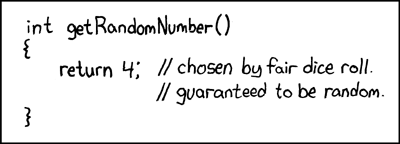
\includegraphics[scale=0.7]{random_number.png}
\end{frame}

\begin{frame}
\frametitle{References}
\footnotesize{
\begin{thebibliography}{99}
 \bibitem[1]{ECDSA}  Don Johnson, Alfred Menezes, Scott Vanstone,
 \newblock The Elliptic Curve Digital Signature Algorithm (ECDSA)
 \newblock \emph{Certicom Research}
  \bibitem[2]{SEC2} Certicom Research
 \newblock SEC 2: Recommended Elliptic Curve Domain Parameters
 \newblock \emph{Certicom Research}
  \bibitem[3]{BERN}  Daniel J. Bernstein, Tanja Lange
 \newblock Analysis and optimization of elliptic-curve single-scalar multiplication
  \bibitem[4]{BPOOL} Brainpool
 \newblock ECC Brainpool Standard Curves and Curve Generation v1.0
 \newblock \emph{Brainpool}
\end{thebibliography}
}
\end{frame}
 
\begin{frame}
\frametitle{References}
\footnotesize{
\begin{thebibliography}{99}
  \bibitem[5]{PAAR}  Chrisoft Paar, Jan pelzl,
 \newblock Understanding Cryptography: A textbook for Students and Practitioners
 \newblock \emph{Springer}
  \bibitem[6]{SUN}  Vipul Gupta, Douglas Stebila, Stephen Fung, Sheueling Chang, Nils Gura, Hans Eberle
 \newblock Speeding up secure web transactions using elliptic curve cryptography
 \newblock \emph{Sun Microsystems Labs}
   \bibitem[7]{PS3}  bushing, marcan, sgher, sven
 \newblock PS3 Epic Fail
 \newblock \emph{fail0verflow}
\end{thebibliography}
}
\end{frame}

 
\begin{frame}
\begin{block}
{Fork here!}
https://github.com/zoep/ECC-OCaml
\end{block}
\bigskip
\begin{block}
{The end}
\end{block}
\end{frame}
% End of slides
\end{document} 